\documentclass{beamer}

% \usetheme[width=3cm]{tuw}
\usetheme{Madrid}

\AtBeginSection[]{
	\begin{frame}
	\vfill
	\centering
		\begin{beamercolorbox}[sep=8pt,center,shadow=true,rounded=true]{title}
			\usebeamerfont{title}\insertsectionhead\par%
		\end{beamercolorbox}
	\vfill
	\end{frame}
}

\usepackage{hyperref}
\usepackage[acronym,toc,nonumberlist]{glossaries}
\usepackage{appendixnumberbeamer}
\usepackage{booktabs}
\usepackage{multirow} 
\usepackage{listings}
\lstset
{ %Formatting for code in appendix
	basicstyle=\footnotesize,
	numbers=left,
	stepnumber=1,
	showstringspaces=false,
	tabsize=1,
	breaklines=true,
	breakatwhitespace=false,
}



\title[Edge Blockchain Provisioning for MEC Apps]{Edge Blockchain Provisioning for Mobile Edge Computing Applications}

\subtitle{Diploma Thesis Presentation}

\author[Filip Rydzi] {BSc Filip Rydzi\\{\small Advisor: Privatdoz. Dr.techn. Hong-Linh Truong}}
\institute[Informatics, TU Wien] {Faculty of Informatics, TU Wien \\
	\vspace{0.3cm}
	
\includegraphics[width=0.3\textwidth]{figures/TU_logo.png}}

% \titlegraphic{
\includegraphics[width=0.3\textwidth]{figures/TU_logo.png}}


\date{\today}

\newacronym{MEC}{MEC}{Mobile Edge Computing}
\newacronym{IoT}{IoT}{Internet of Things}
\newacronym{V2X}{V2X}{Vehicle-to-Everything}
\newacronym{RSU}{RSU}{Road-side unit}
\newacronym{TOSCA}{TOSCA}{Topology and Orchestration Specification for Cloud Applications}

\begin{document}
	
	\begin{frame}
		\titlepage
	\end{frame}

	\begin{frame}
		\frametitle{Overview}
		\tableofcontents
	\end{frame}

	\section{Introduction \& Motivation}
	
	\begin{frame}
		\frametitle{Introduction}
		
		\begin{columns}[t]
			\begin{column}{.5\textwidth}
				\textbf{\gls{MEC}}
				\begin{itemize}
					\item An architecture, which brings cloud capabilities (processing, storage, etc.) closer to the users.
					\item Additional layer between cloud and \gls{IoT}.
				\end{itemize}
				\only<2>{
					\textbf{Blockchain for \gls{MEC}}
					\begin{itemize}
						\item Decentralized trust-less peer-to-peer messaging solution.
						\item Autonomous management of \gls{IoT} devices.
					\end{itemize}
				}
			\end{column}
			
			\begin{column}{.5\textwidth}
				\only<1>{
					\begin{figure}
						\centering
						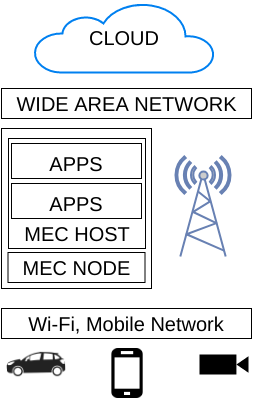
\includegraphics[width=0.5\textwidth]{figures/mec_overview0.png}
						\caption{\gls{MEC} architectural overview, taken from \cite{dolui17}}
					\end{figure}
				}
				\only<2>{
					\begin{figure}
						\centering
						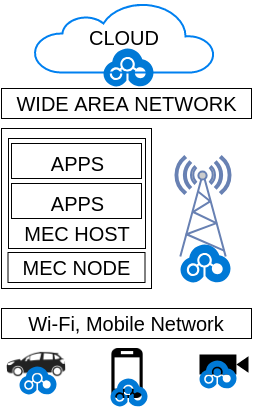
\includegraphics[width=0.5\textwidth]{figures/mec_overview.png}
						\caption{\gls{MEC} with blockchain architectural overview, taken from \cite{dolui17}}
					\end{figure}
				}
			\end{column}
			
		\end{columns}
		
	\end{frame}
	
	
	\begin{frame}
		\frametitle{Motivation Scenario}
		
		\only<1>{
			\begin{figure}
				\centering
				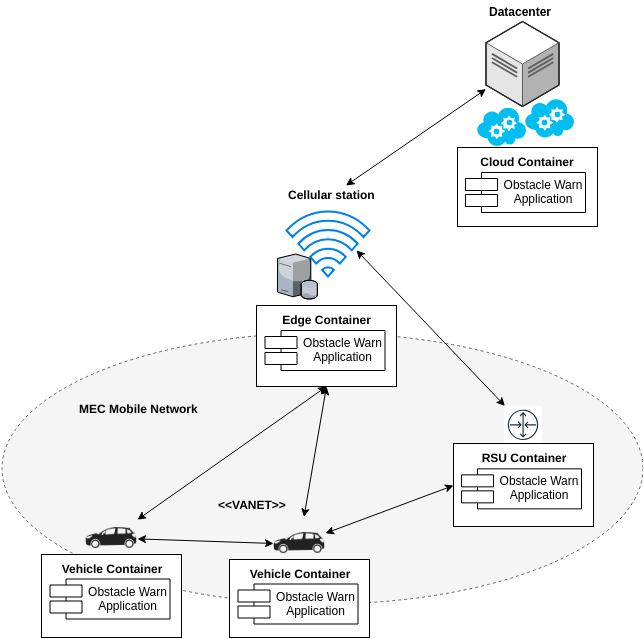
\includegraphics[width=0.6\textwidth]{figures/motivation_scenario1.png}
				\caption{Motivation Scenario}
			\end{figure}
		}
		\only<2>{
			\begin{figure}
				\centering
				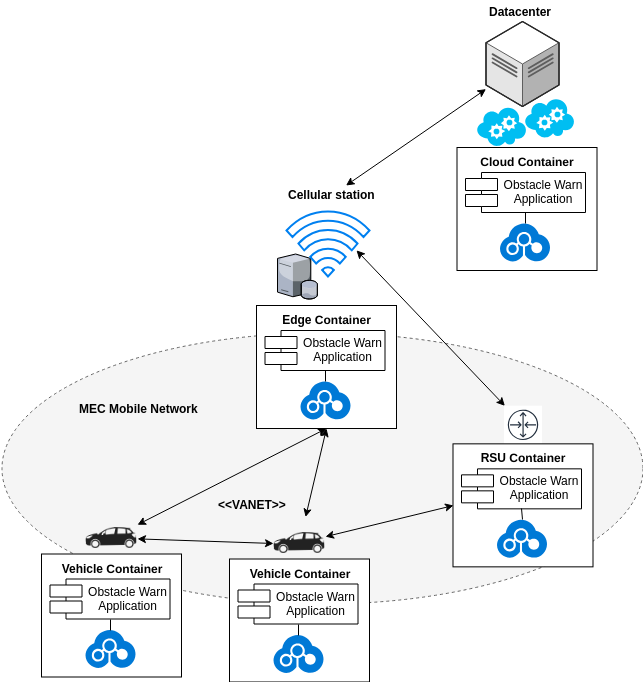
\includegraphics[width=0.6\textwidth]{figures/motivation_scenario2.png}
				\vspace{-0.5cm}
				\caption{Motivation Scenario}
			\end{figure}
		}
		\only<3>{
			\begin{figure}
				\centering
				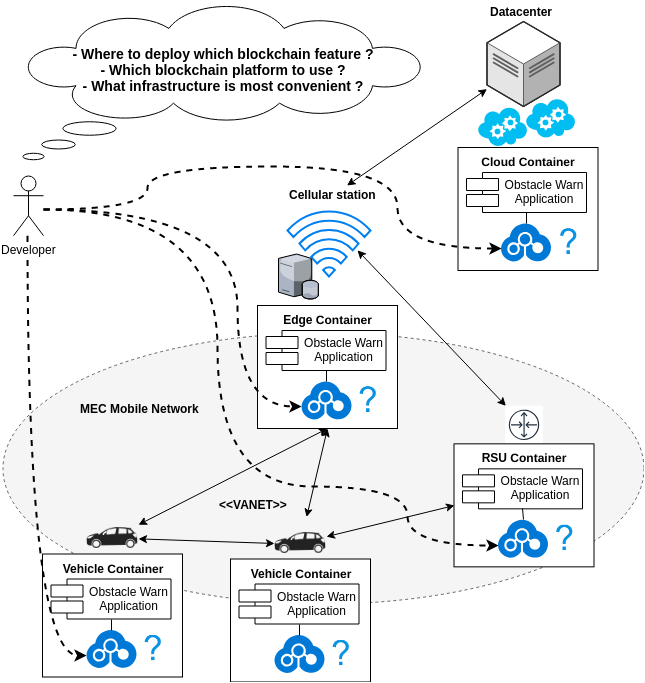
\includegraphics[width=0.6\textwidth]{figures/motivation_scenario.png}
				\vspace{-0.5cm}
				\caption{Motivation Scenario}
			\end{figure}
		}
		
	\end{frame}
	
	
	\begin{frame}
		\frametitle{Research Objectives}
		\begin{enumerate}
			\item Benchmark different patterns of blockchain interactions among \gls{MEC} components. Evaluate various deployments of blockchain artefacts to the components and various configurations of infrastructure, consisting of compute resources and networks.
			\item Provide knowledge gathered by the benchmarks to the developers.
		\end{enumerate}
	\end{frame}


	\begin{frame}
		\frametitle{Contribution}
		\begin{itemize}
			\item Benchmark Framework
			\begin{itemize}
				\item Benchmark blockchain interactions among \gls{MEC} components in an application's topology.
			\end{itemize}
			\item Experiment Knowledge Service
			\begin{itemize}
				\item Manage knowledge gathered by benchmarks to help developers during design phase of an application.
			\end{itemize}
		\end{itemize}
	\end{frame}
	
	\section{Benchmarks}
	
	\begin{frame}
		\frametitle{Quality Metrics}
		\begin{itemize}
			\item Transaction Acceptance Rate
			\begin{itemize}
				\item The ratio of accepted transactions to the ones which have been submitted to blockchain.
			\end{itemize}
			\item Transaction Acceptance Time
			\begin{itemize}
				\item The time it takes to accept a transaction by blockchain.
			\end{itemize}
			\item Synchronization State
			\item Scalability
			\item Infrastructure Resources Utilization
		\end{itemize}
	\end{frame}
		
	\begin{frame}
		\frametitle{Scenarios and Interactions}
			\textbf{Examples of interaction patterns:}
			\begin{enumerate}
				\item Vehicle to Vehicle Interaction
				\item \textbf<2>{Vehicle to \gls{RSU} Interaction}
				\only<2> {
					\begin{itemize}
						\item \textit{Obstacle on the road warning scenario}
					\end{itemize}
				}
				
				\item Vehicle to Edge Interaction
				\item Vehicle to \gls{RSU} and Edge Interaction
				\item Vehicle to Edge and Cloud Interaction
				\item Vehicle to \gls{RSU}, Edge and Cloud Interaction
			\end{enumerate}
	\end{frame}

	\begin{frame}
		\frametitle{Benchmarks Design}
		
		\begin{table}
			\centering
			\caption{A deployment of blockchain features for Interaction 2 (vehicle-\gls{RSU}-vehicle)}
			\label{tab:bc_deployment_interaction2}
			\resizebox{0.5\textwidth}{!}{
				\begin{tabular}{|c|c|c|c|c|c|} 
					\hline
					\textbf{Interaction id}      & \multicolumn{5}{c|}{\textbf{Blockchain features deployment}}                               \\ 
					\hline
					\multirow{4}{*}{\textbf{2} } & \textbf{ID}  & \textbf{vehicle}  & \textbf{\gls{RSU}}        & \textbf{Edge}  & \textbf{Cloud}   \\ 
					\cline{2-6}
					& 0            & \textit{creator}  & \textit{all}        & \textit{-}     & \textit{-}       \\ 
					\cline{2-6}
					& 2            & \textit{all}      & \textit{creator}    & \textit{-}     & \textit{-}       \\ 
					\cline{2-6}
					& 4            & \textit{all}      & \textit{all}        & \textit{-}     & \textit{-}       \\
					\hline
				\end{tabular}
			}
		\end{table}
	
		\textbf{Blockchain features}
		\begin{itemize}
			\item \textit{Creator feature} (creating, signing, submitting and verifying a transaction, accepting a block)
			\item \textit{Consensus feature} (achieve consensus)
		\end{itemize}
	
	\end{frame}
		
		\begin{frame}
			\frametitle{Benchmark Framework}
			
			\begin{figure}[h]
				\centering
				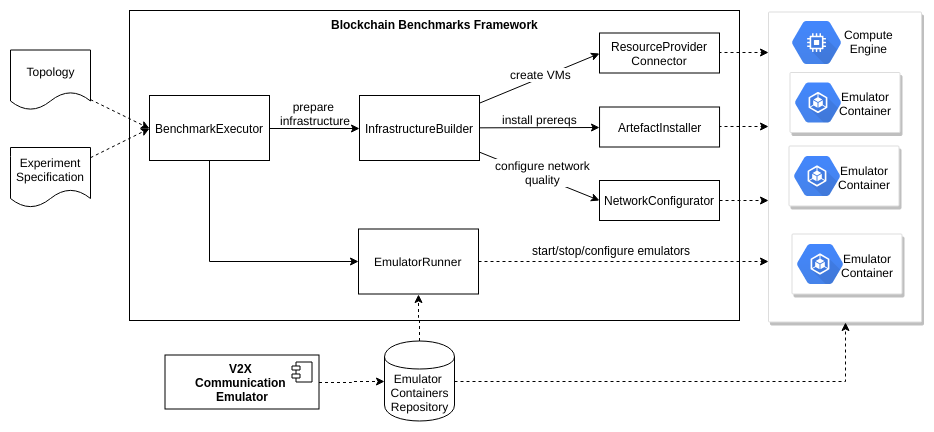
\includegraphics[width=0.9\textwidth]{figures/benchmark_framework_component_diagram.png}
				\vspace{-0.5cm}
				\caption{Component diagram of the framework}
				\label{fig:benchmark_framework_component}
			\end{figure}
			
			\vspace{-0.5cm}
			\begin{itemize}
				\item Generate and benchmark experiments based on a specification.
				\item Build emulated MEC infrastructure.
				\item Deploy blockchain artefacts into a specified topology.
				\item Emulate and benchmark blockchain interactions among MEC components in the topology.
			\end{itemize}
		
		\end{frame}
		
		\begin{frame}
			\frametitle{Experiments}
			\begin{itemize}
				\item 324 experiments have been generated and benchmarked by the benchmark framework.
			\end{itemize}
			
			\begin{figure}
				\centering
				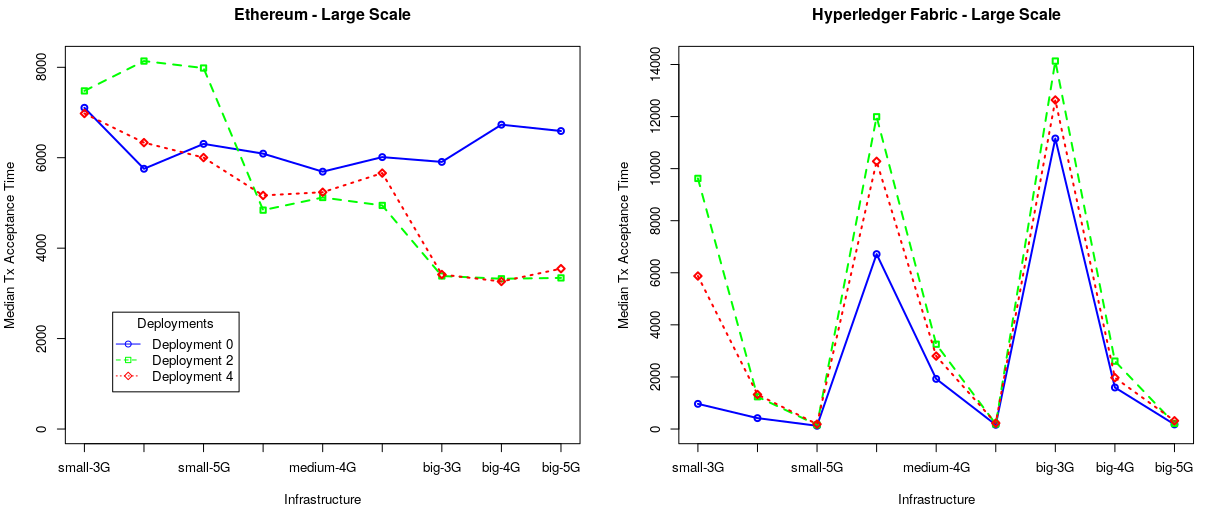
\includegraphics[width=\textwidth]{figures/interaction2_large_scale_median_times.png}
				\vspace{-0.5cm}
				\caption{Median of transaction acceptance times for interaction 2 (vehicle-\gls{RSU}-vehicle)}
				\label{fig:experiments1}
			\end{figure}
		
		\end{frame}
		
		\begin{frame}
			\frametitle{Experiments - Discussion}
			\begin{itemize}
			\item All identified interactions for the \textit{obstacle on the road warning scenario} have been benchmarked.
				\begin{enumerate}
					\setcounter{enumi}{1}
					\item Vehicle to \gls{RSU} Interaction
					\item Vehicle to Edge Interaction
					\item Vehicle to \gls{RSU} and Edge Interaction
				\end{enumerate}
			\item Best results concerning reliability and performance have been measured for: \textit{interaction 2, Hyperledger-Fabric blockchain, deployment 0, small machine type for vehicles and 5G network }.
			\end{itemize}
		\end{frame}
	
	
	\section{Experiments Knowledge Service}
	
	\begin{frame}
		\frametitle{Overview}
		\begin{figure}[h]
			\centering
			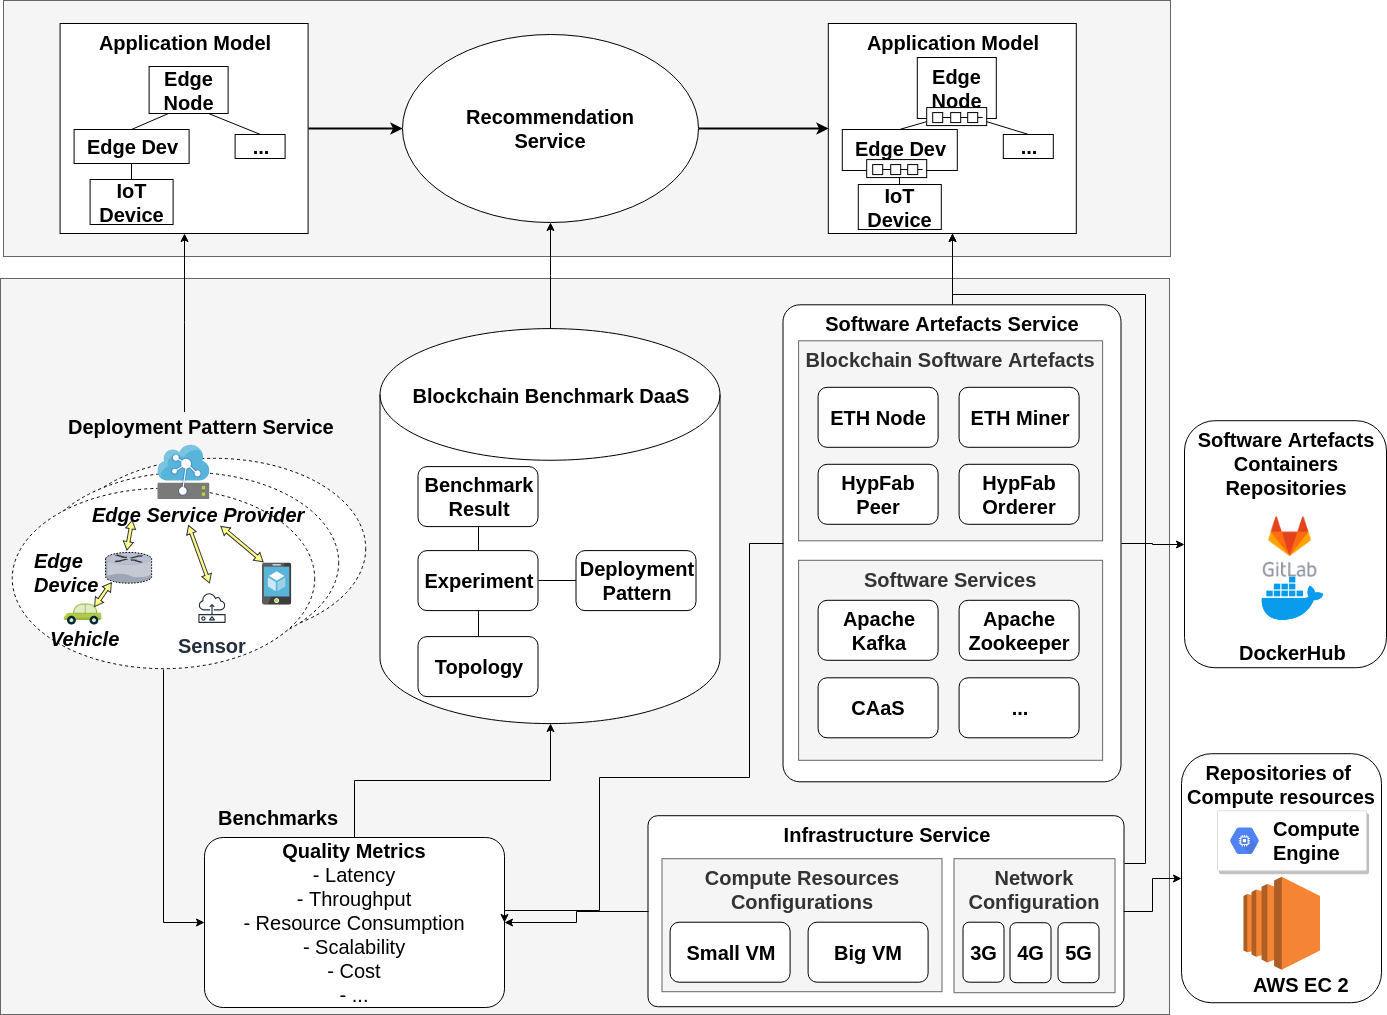
\includegraphics[width=0.7\textwidth]{figures/knowledge_service_high_level_architecture.png}
			\caption{High-level architectural overview of Experiments Knowledge Service}
			\label{fig:experiments_knowledge_service_overview}
		\end{figure}
		
	\end{frame}
	
	\begin{frame}
		\frametitle{Data model}
		\begin{figure}[h]
		\centering
			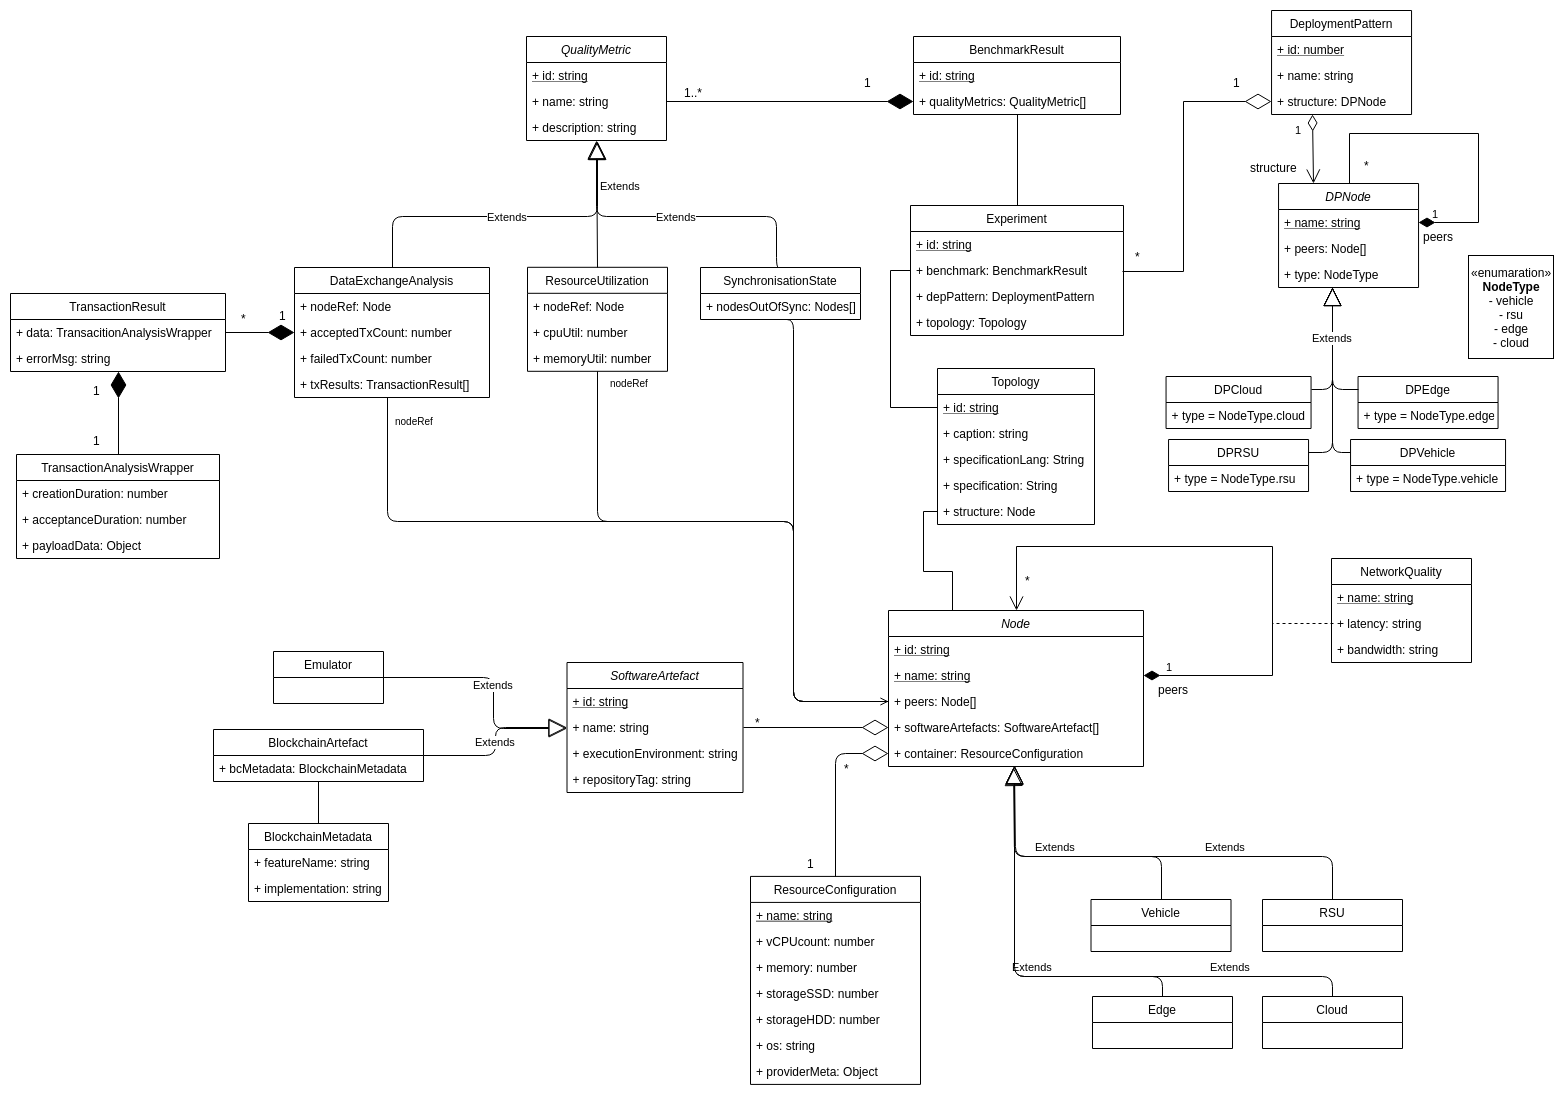
\includegraphics[width=0.9\textwidth]{figures/benchmarked_experiment_data_model_portrain.png}
			\vspace{-0.5cm}
			\caption{Model of data stored in Experiments Knowledge Service}
			\label{fig:benchmarked_experiment_model}
		\end{figure}
	\end{frame}

	\begin{frame}
		\frametitle{Features}
		
	
		\begin{itemize}
			\item Sharing benchmarks with the Experiment Knowledge Service.
			\item Search benchmarking interactions, topologies or infrastructures.
			\item Recommend a deployment of blockchain artefacts into a model of application in \gls{MEC}.
		\end{itemize}
	
	\end{frame}
	
	\begin{frame}
		\frametitle{Examples}
			
			\begin{columns}[t]
				\begin{column}{.5\textwidth}
					\begin{figure}[h]	
						\centering
						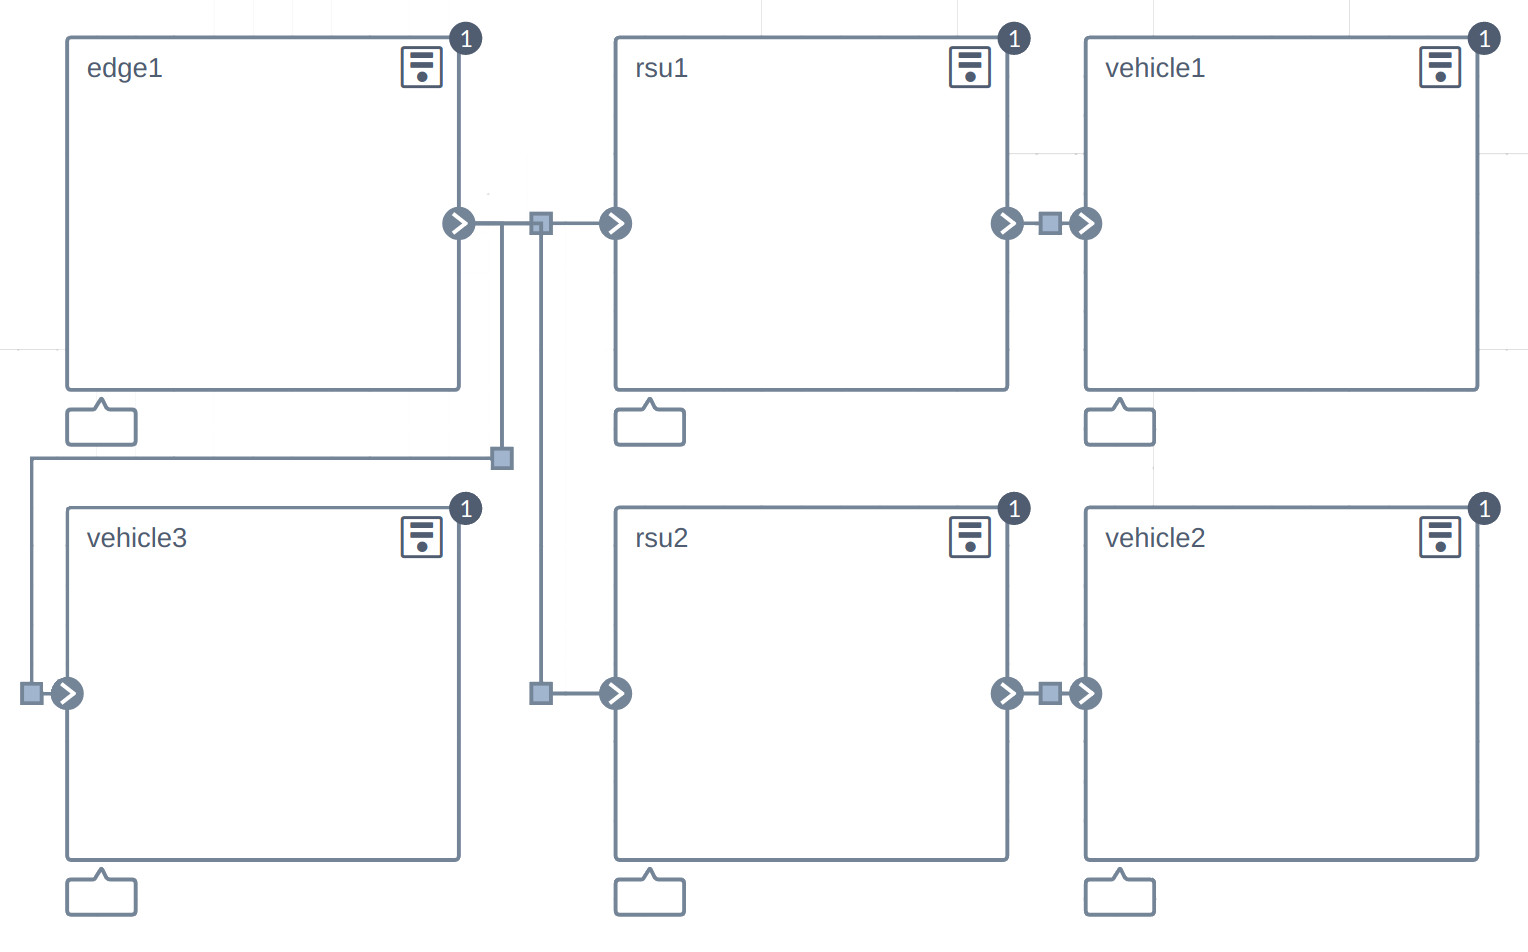
\includegraphics[width=1\textwidth]{figures/tosca_input.png}
						\caption{Input for Recommendation Service, depicted via Cloudify Composer \protect\footnotemark}
						\label{fig:recommendation_example_input}
					\end{figure}
				\end{column}
			
				\begin{column}{.5\textwidth}
					\begin{figure}[h]	
						\centering
						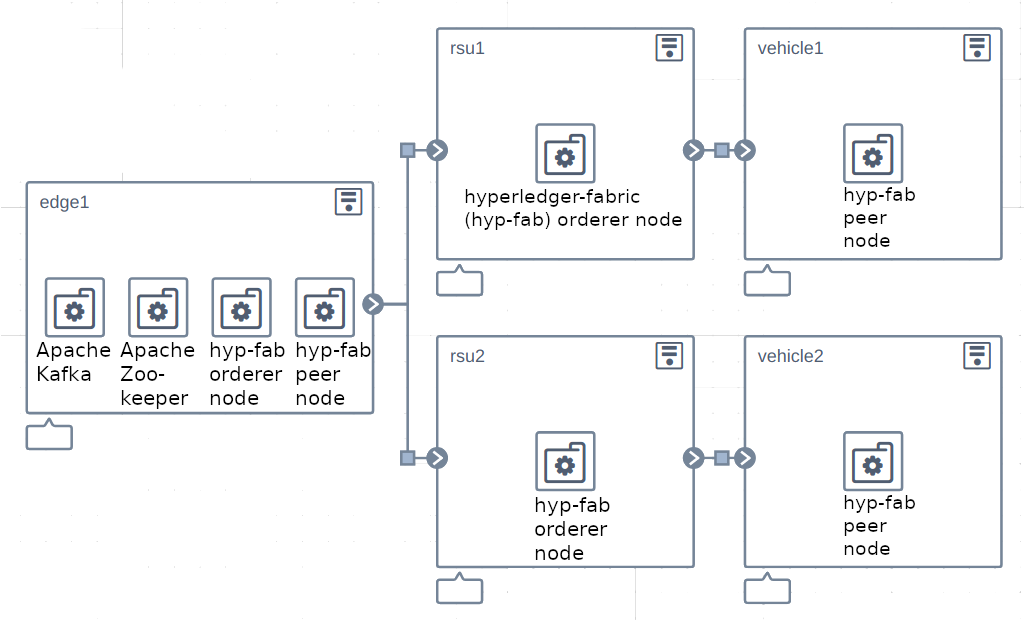
\includegraphics[width=1\textwidth]{figures/tosca_output.png}
						\caption{Output from Recommendation Service, depicted via Cloudify Composer}
						\label{fig:recommendation_example_output}
					\end{figure}
				\end{column}
				
			\end{columns}
		
			\footnotetext{\url{https://docs.cloudify.co/4.5.0/developer/composer/}}
	
	\end{frame}
	
	\section{Prototype \& Demo}
	
	\begin{frame}
		\frametitle{Prototypes \& Demo}
		\begin{itemize}
			\item Benchmark Framework
			\begin{itemize}
				\item Dockerized NodeJS application, developed in Typescript.
			\end{itemize}
			\item Experiment Knowledge Service
			\begin{itemize}
				\item Dockerized NodeJS application, developed in Typescript, stores data in MongoDB and Neo4J.
			\end{itemize}
		\end{itemize}
		The prototypes are available in the GitHub repository \footnote{\url{https://github.com/rdsea/blockchainbenmarkservice}}.
	
	\end{frame}
	
	\section{Conclusions \& Future Works}

	\begin{frame}
		\frametitle{Conclusions}
		
		\begin{itemize}
			\item Blockchain in \gls{MEC} brings new challenges for developers.
			\item To help the developers we introduced a framework able to benchmark blockchain interactions among \gls{MEC} components.
			\item 324 experiments have been performed to demonstrate flexibility of the framework.
			\item To enable reuse of the knowledge gathered by benchmarks we developed an Experiments Knowledge Service.
		\end{itemize}
		
	\end{frame}

	\begin{frame}
		\frametitle{Current \& Future Works}
		
		\textbf{Contribution Papers:}
		\begin{itemize}
			\item Benchmarking Blockchain Interactions in Mobile Edge Cloud Software Systems
			\begin{itemize}
				\item submitted to IEEE MASCOTS 2019 \footnote{\url{https://sites.google.com/view/mascots-2019}}
			\end{itemize}
			\item Sharing Blockchain Performance Knowledge for Edge Service Development
			\begin{itemize}
				\item submitted to ICSOC 2019 \footnote{\url{https://icsoc-laas.fr/}}
			\end{itemize}
		\end{itemize}
		
	\end{frame}

	\begin{frame}
		\frametitle{References}
		\bibliographystyle{plain}
		\bibliography{references}
	\end{frame}

	\appendix
	
	\section{Backup slides}
	
	\begin{frame}
	\frametitle{Quality Metrics}
		\begin{itemize}
			\item Transaction Acceptance Rate
			\begin{itemize}
				\item The ratio of accepted transactions to the ones which have been submitted to blockchain.
			\end{itemize}
			\item Synchronization State
			\begin{itemize}
				\item The number of blockchain nodes, which have been removed from a blockchain’s topology
				during a period of time.
			\end{itemize}
			\item Transaction Acceptance Time
			\begin{itemize}
				\item The time it takes to accept a transaction by blockchain.
			\end{itemize}
			\item Scalability
			\begin{itemize}
				\item Changes in transaction acceptance rate and time and in synchronization state when scale of a topology is increased.
			\end{itemize}
			\item Infrastructure Resources Utilization
			\begin{itemize}
				\item \% utilization of a CPU core, RAM memory, etc.
			\end{itemize}
		\end{itemize}
	\end{frame}

	\begin{frame}
		\frametitle{Vehicle to Vehicle Interaction}
		\begin{figure}
			\centering
			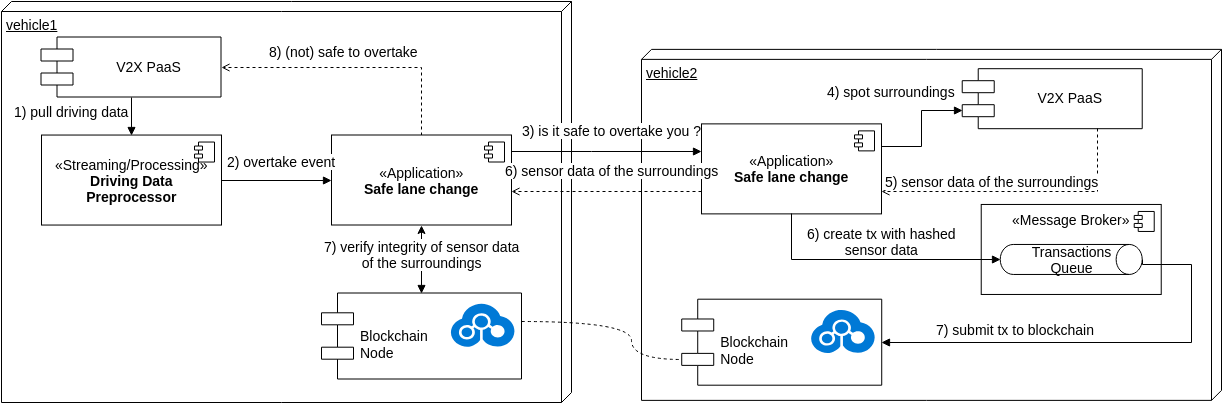
\includegraphics[width=0.9\textwidth]{figures/bc_interactions/bc_v2v_interaction.png}
			\caption{Lane Change Scenario in a blockchain-enabled \gls{V2X} communication}
			\label{fig:interaction_v2v}
		\end{figure}
	\end{frame}

	\begin{frame}
		\frametitle{Vehicle to \gls{RSU} Interaction}
		\begin{figure}
			\centering
			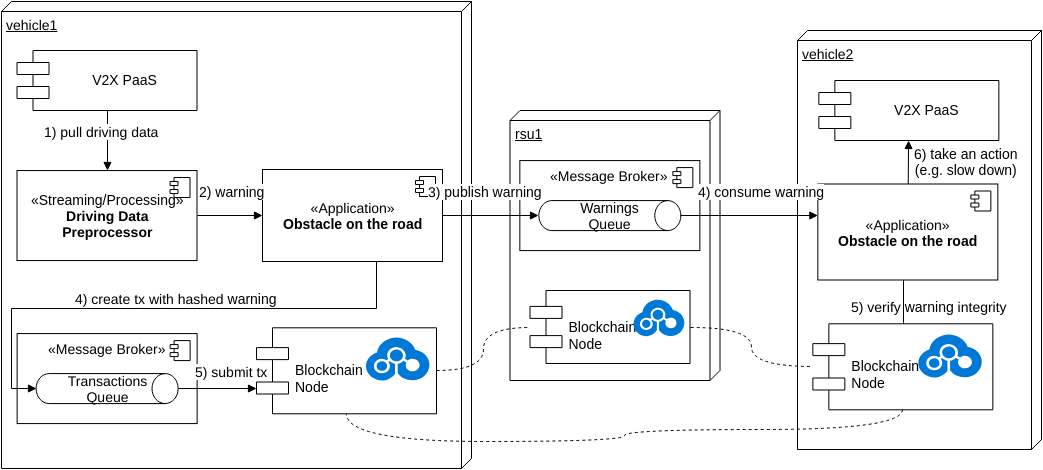
\includegraphics[width=0.9\textwidth]{figures/bc_interactions/bc_interaction_veh_rsu_veh.png}
			\caption{The \textit{obstacle on the road warning scenario} in blockchain-enabled \gls{V2X} over \gls{RSU}}
			\label{fig:interaction_v2x_rsu}
		\end{figure}
	\end{frame}

	\begin{frame}
		\frametitle{Vehicle to Edge Interaction}
		\begin{figure}
			\centering
			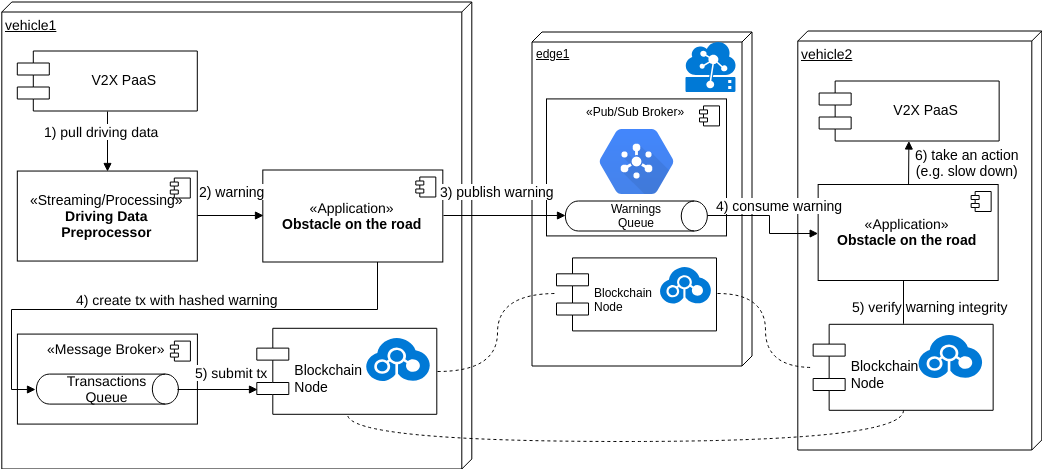
\includegraphics[width=0.9\textwidth]{figures/bc_interactions/bc_interaction_veh_edge_veh.png}
			\caption{The \textit{obstacle on the road warning scenario} in blockchain-enabled \gls{V2X} over edge node}
			\label{fig:interaction_v2x_edge}
		\end{figure}
	\end{frame}

	\begin{frame}
		\frametitle{Vehicle to \gls{RSU} and Edge Interaction}
		\begin{figure}
			\centering
			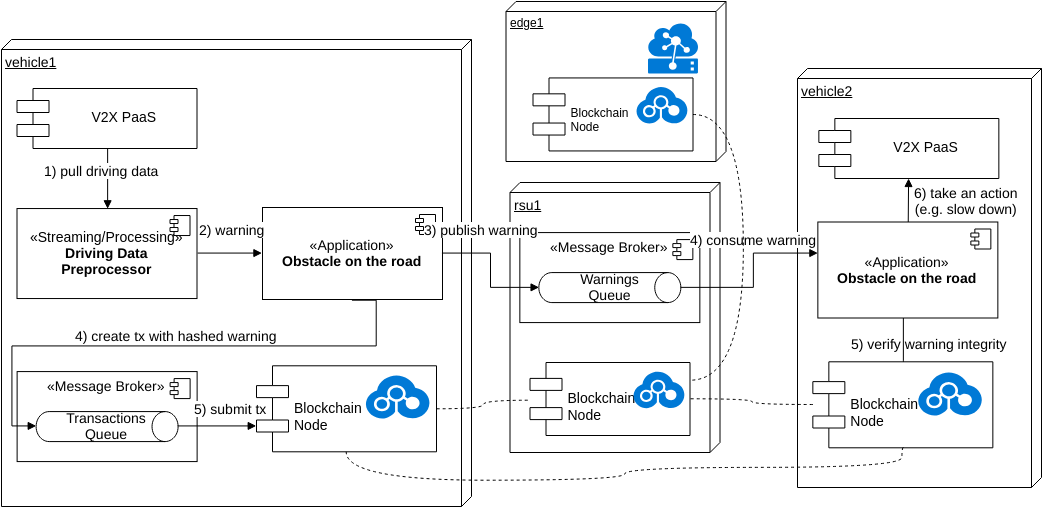
\includegraphics[width=0.9\textwidth]{figures/bc_interactions/bc_interaction_veh_rsu_edge_veh.png}
			\caption{The \textit{obstacle on the road warning scenario} in blockchain-enabled \gls{V2X} over \gls{RSU} and edge node}
			\label{fig:interaction_v2x_rsu_edge}
		\end{figure}
	\end{frame}

	\begin{frame}
		\frametitle{Blockchain Artefact}
		\textbf{Blockchain features}
		\begin{itemize}
			\item \textit{Creator feature}
			\begin{itemize}
				\item Create a transaction
				\item Sign a transaction
				\item Submit a transaction
				\item Verify a transaction
				\item Accept a block
			\end{itemize}
			\item \textit{Consensus feature}
			\begin{itemize}
				\item Achieve consensus
			\end{itemize}
		\end{itemize}
		\textbf{Blockchain nodes}
		\begin{itemize}
			\item Standard node
			\begin{itemize}
				\item Capable of executing the \textit{Creator feature}.
				\item Real examples: \texttt{Geth node}, \texttt{Hyperledger-Fabric peer node}
			\end{itemize}
			\item Miner node
			\begin{itemize}
				\item Capable of executing the \textit{Consensus feature}.
				\item Real examples: \texttt{Geth miner node}, \texttt{Hyperledger-Fabric orderer node}
			\end{itemize}
		\end{itemize}
	\end{frame}

	\begin{frame}
		\frametitle{Blockchain Artefacts}
		\begin{figure}
			\centering
			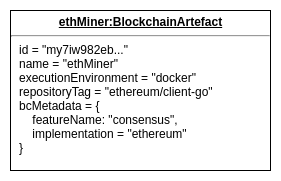
\includegraphics[width=0.5\textwidth]{figures/bc_artefact_example.png}
			\vspace{-0.5cm}
			\caption{Ethereum miner node}
			\label{fig:bc_artefact_example}
		\end{figure}
	\end{frame}

	\begin{frame}
		\frametitle{Benchmark Infrastructure}
		\begin{figure}
			\centering
			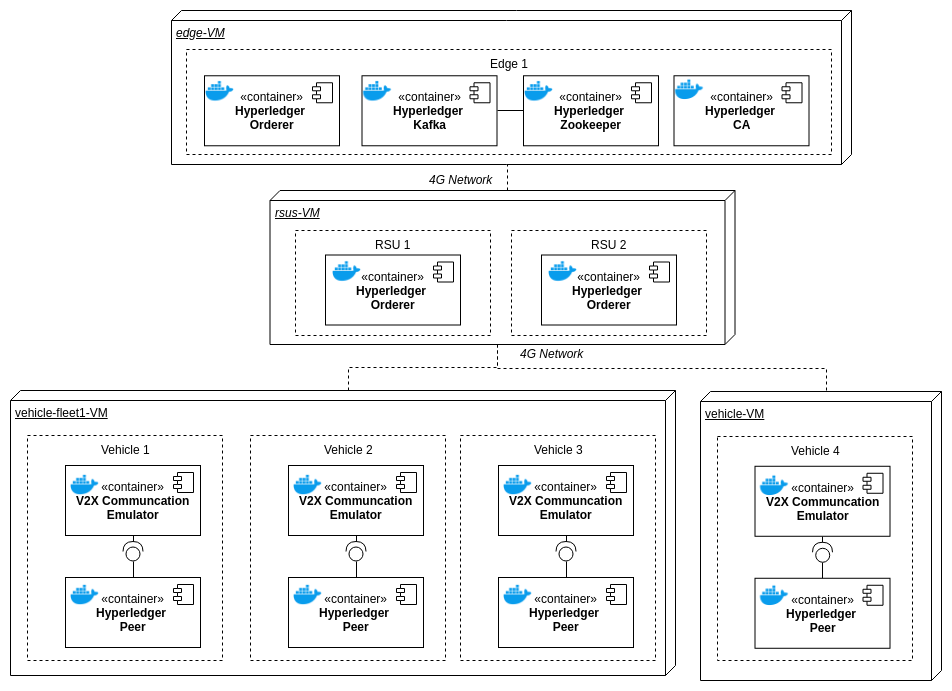
\includegraphics[width=0.8\textwidth]{figures/experiment_deployment_diagram.png}
			\caption{Example of emulated \gls{MEC} infrastructure}
			\label{fig:emulated_mec_infrastructure}
		\end{figure}
	\end{frame}

	\begin{frame}
		\frametitle{Benchmark Framework}
		\begin{figure}
			\centering
			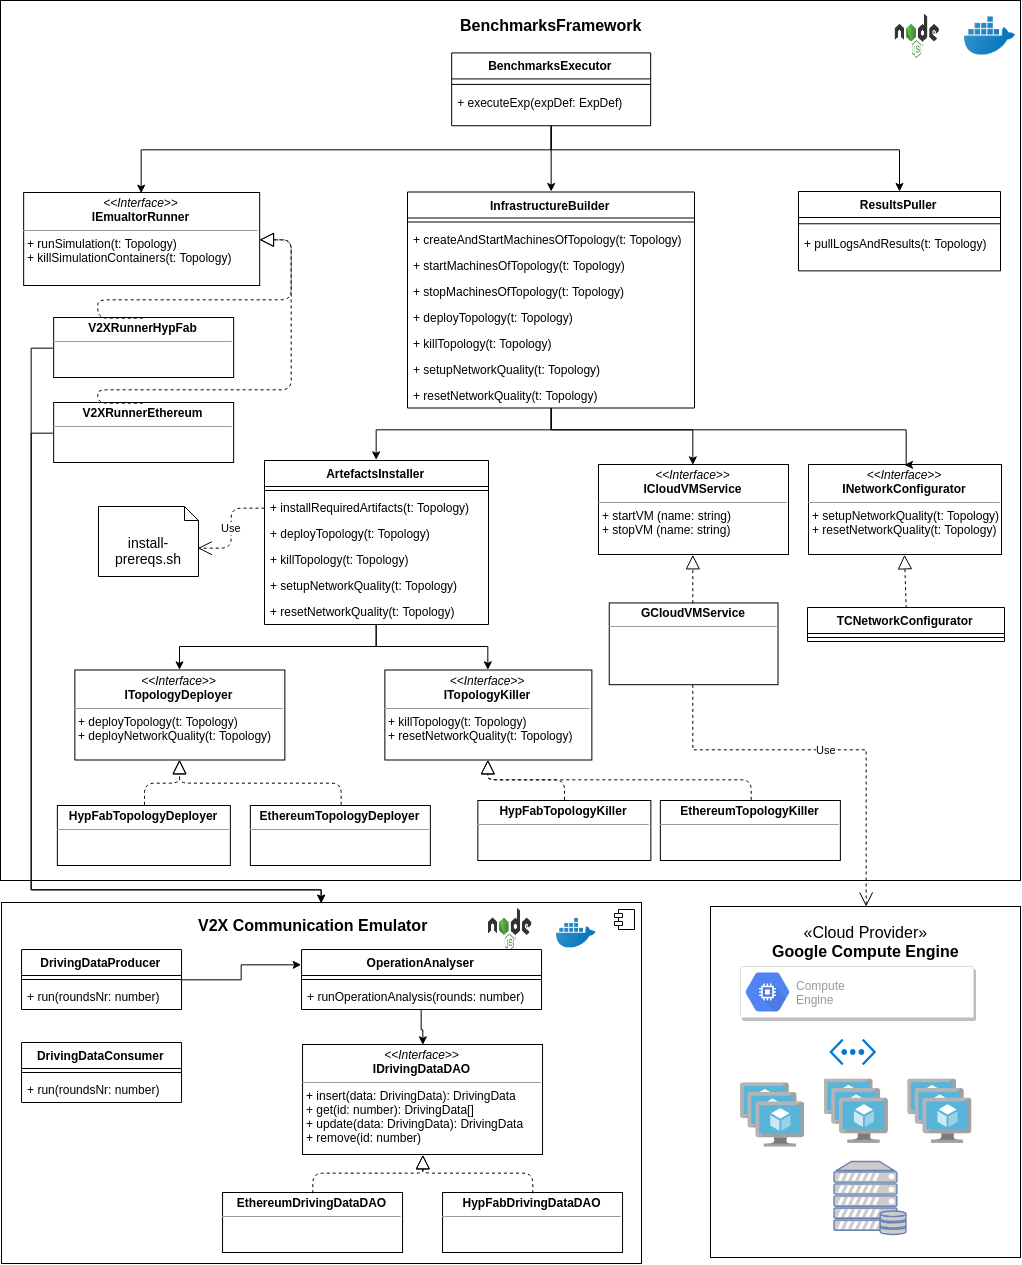
\includegraphics[width=0.5\textwidth]{figures/benchmarks_framework_classes.png}
			\vspace{-0.5cm}
			\caption{Class diagram of the framework}
			\label{fig:benchmark_framework_class}
		\end{figure}
	\end{frame}

	\begin{frame}
		\frametitle{Benchmark Framework - Input Topology}
		\begin{figure}
			\centering
			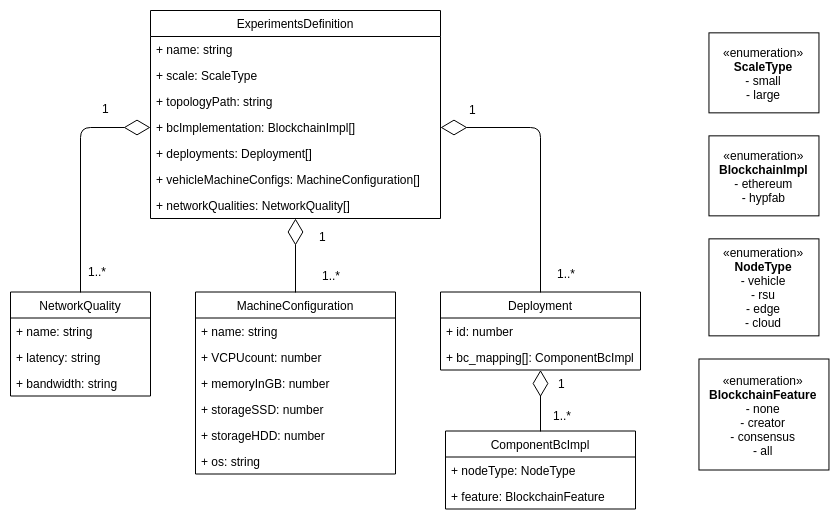
\includegraphics[width=0.8\textwidth]{figures/benchmark_framework_experiment_def.png}
			\vspace{-0.5cm}
			\caption{JSON representation of topology accepted by benchmark framework}
			\label{fig:benchmark_framework_input_topology}
		\end{figure}
	\end{frame}


	\begin{frame}[fragile]
		\frametitle{Benchmark Framework - Experiment Specification}

			\begin{columns}[t]
				\begin{column}{.4\textwidth}
					
					\begin{lstlisting} [frame=single,basicstyle=\ttfamily\scriptsize]
name: interaction2
description: Experiments for Interaction2					
workloadEmulator:
- type: docker
  imageTag: filiprydzi/v2x_communication
  roundsNr: 100					
bcImplementations:
- eth
- hypfab
bcDeployments:
- id: 4
  featuresMapping:
  - nodeType: rsu
    feature: all
  - nodeType: vehicle
    feature: all
...
					\end{lstlisting}
					
				\end{column}
				
				\begin{column}{.4\textwidth}
					
					\begin{lstlisting} [frame=single,basicstyle=\ttfamily\scriptsize,firstnumber=18]
vehicleContainerConfigurations:
- name: small
  vCPUcount: 1
  memory: 2
  storageSSD: 10
  storageHDD: 0
  os: ubuntu18.04
  ...
networkQualities:
- name: 3G
  latency: 200ms
  bandwidth: 1000kbps
  ...
					\end{lstlisting}
					
				\end{column}
			\end{columns}		
	\end{frame}

	\begin{frame}
		\frametitle{Experiments}
		
		\begin{figure}
			\centering
			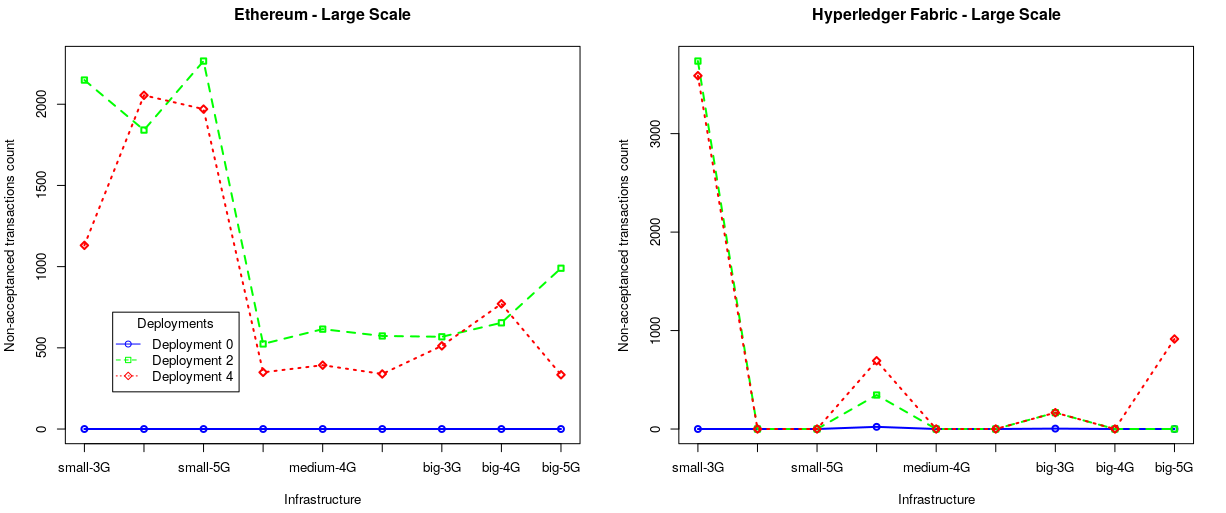
\includegraphics[width=\textwidth]{figures/interaction2_rejected_tx.png}
			\vspace{-0.5cm}
			\caption{Number of rejected transactions in interaction 2 (vehicle-\gls{RSU}-vehicle)}
			\label{fig:experiments0}
		\end{figure}
		
	\end{frame}


	\begin{frame}
		
		\begin{figure}
			\centering
			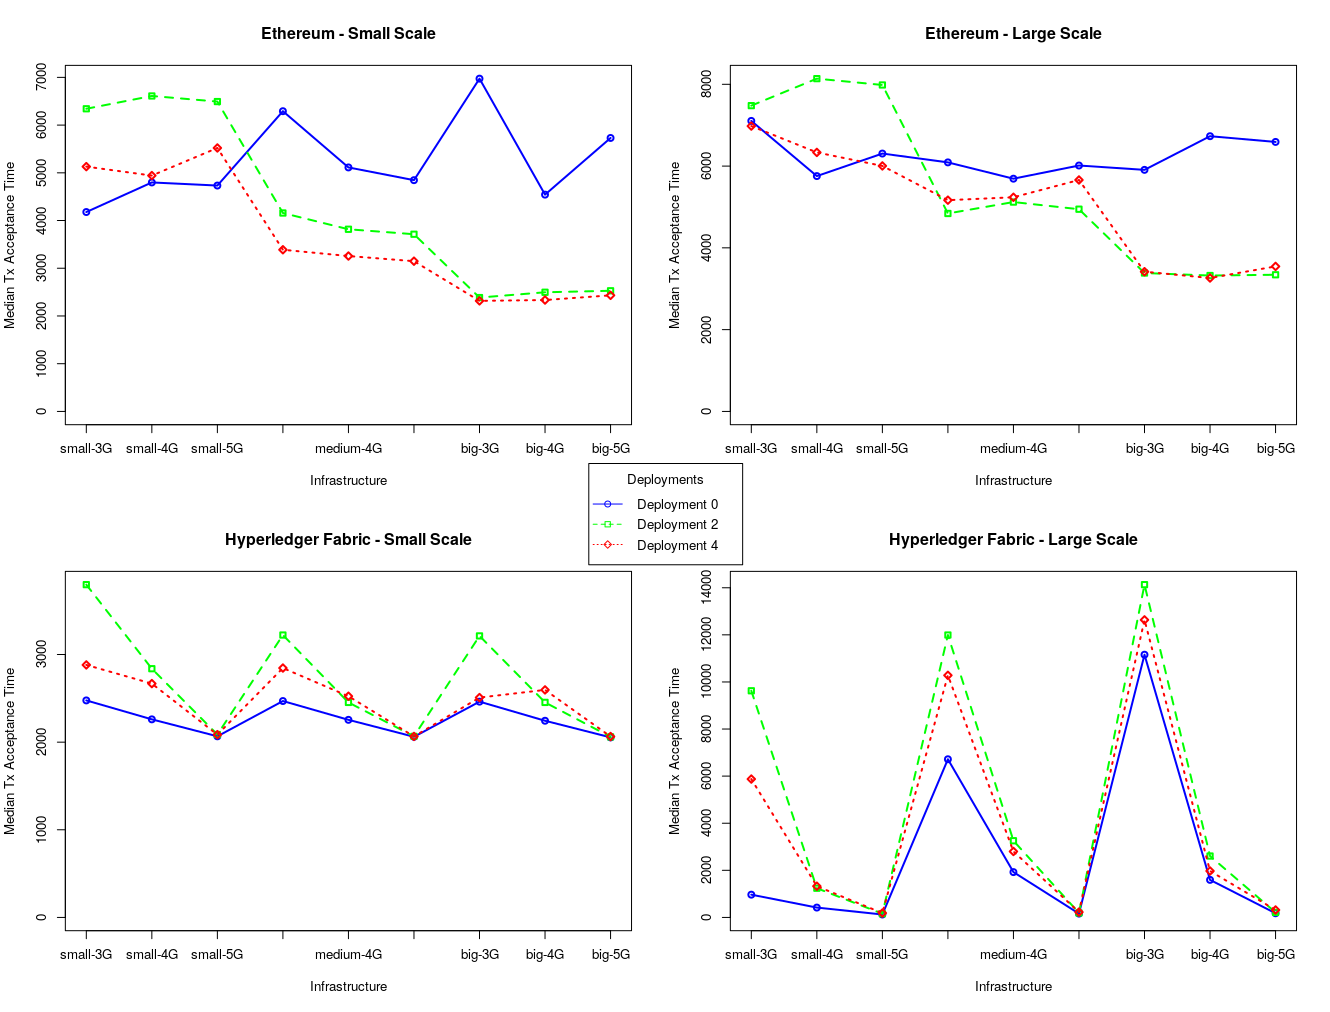
\includegraphics[width=0.8\textwidth]{figures/interaction2_median_accept_time.png}
			\vspace{-0.5cm}
			\caption{Median of transaction acceptance times for interaction 2 (vehicle-\gls{RSU}-vehicle)}
			\label{fig:experiments}
		\end{figure}
		
	\end{frame}

	\begin{frame}
		\frametitle{Experiments}
		
		\begin{figure}
			\centering
			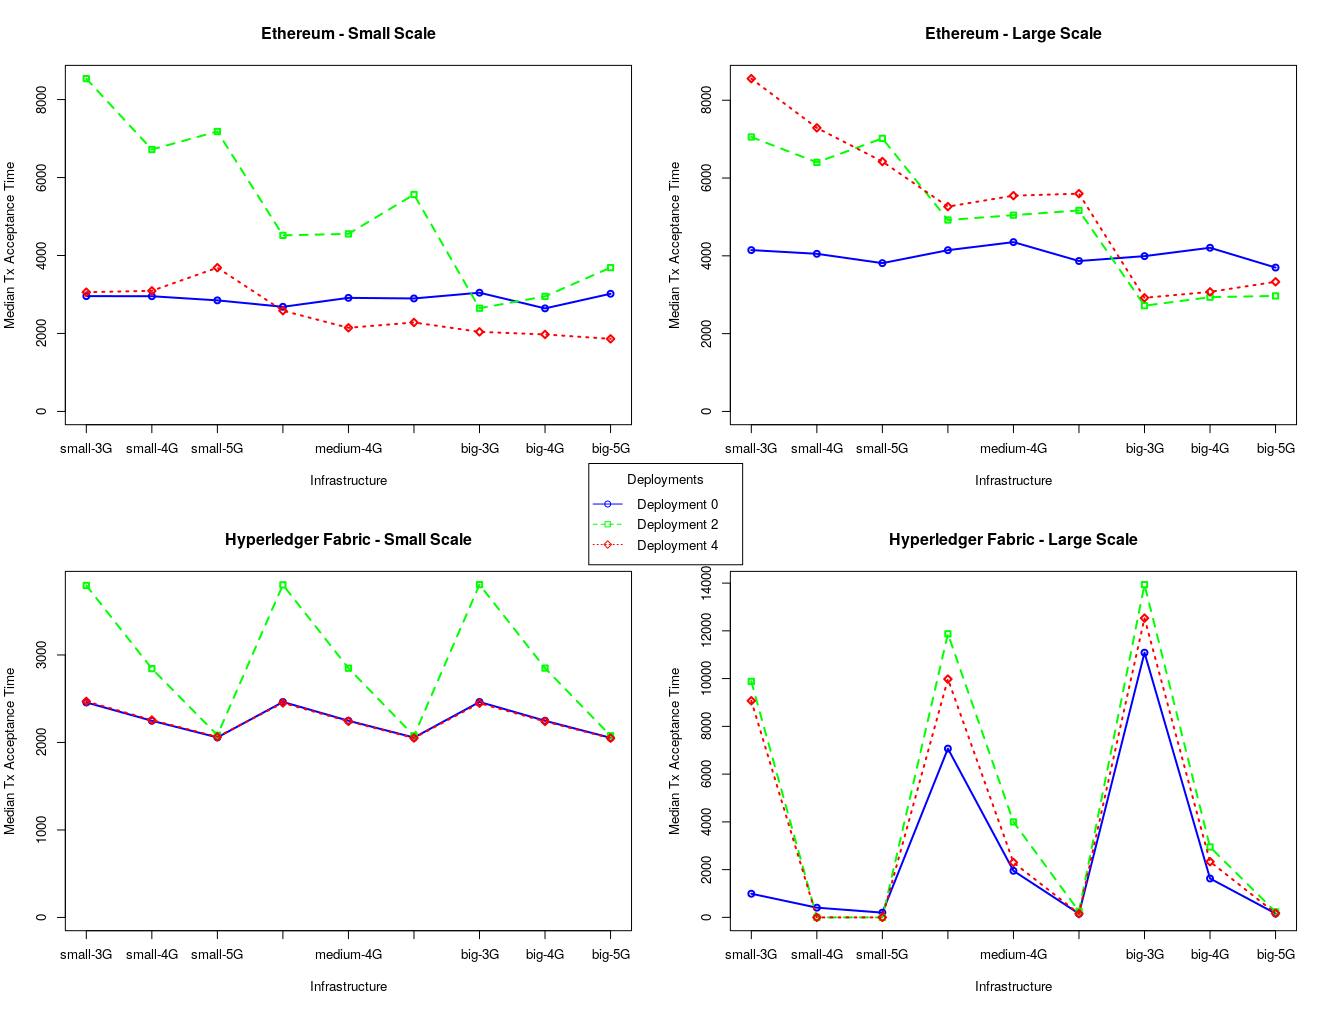
\includegraphics[width=0.8\textwidth]{figures/interaction3_median_accept_time.png}
			\vspace{-0.5cm}
			\caption{Median of transaction acceptance times for interaction 3 (vehicle-edge node-vehicle)}
			\label{fig:experiments3}
		\end{figure}
		
	\end{frame}
	
	
	\begin{frame}
		\frametitle{Experiments}
		
		\begin{figure}
			\centering
			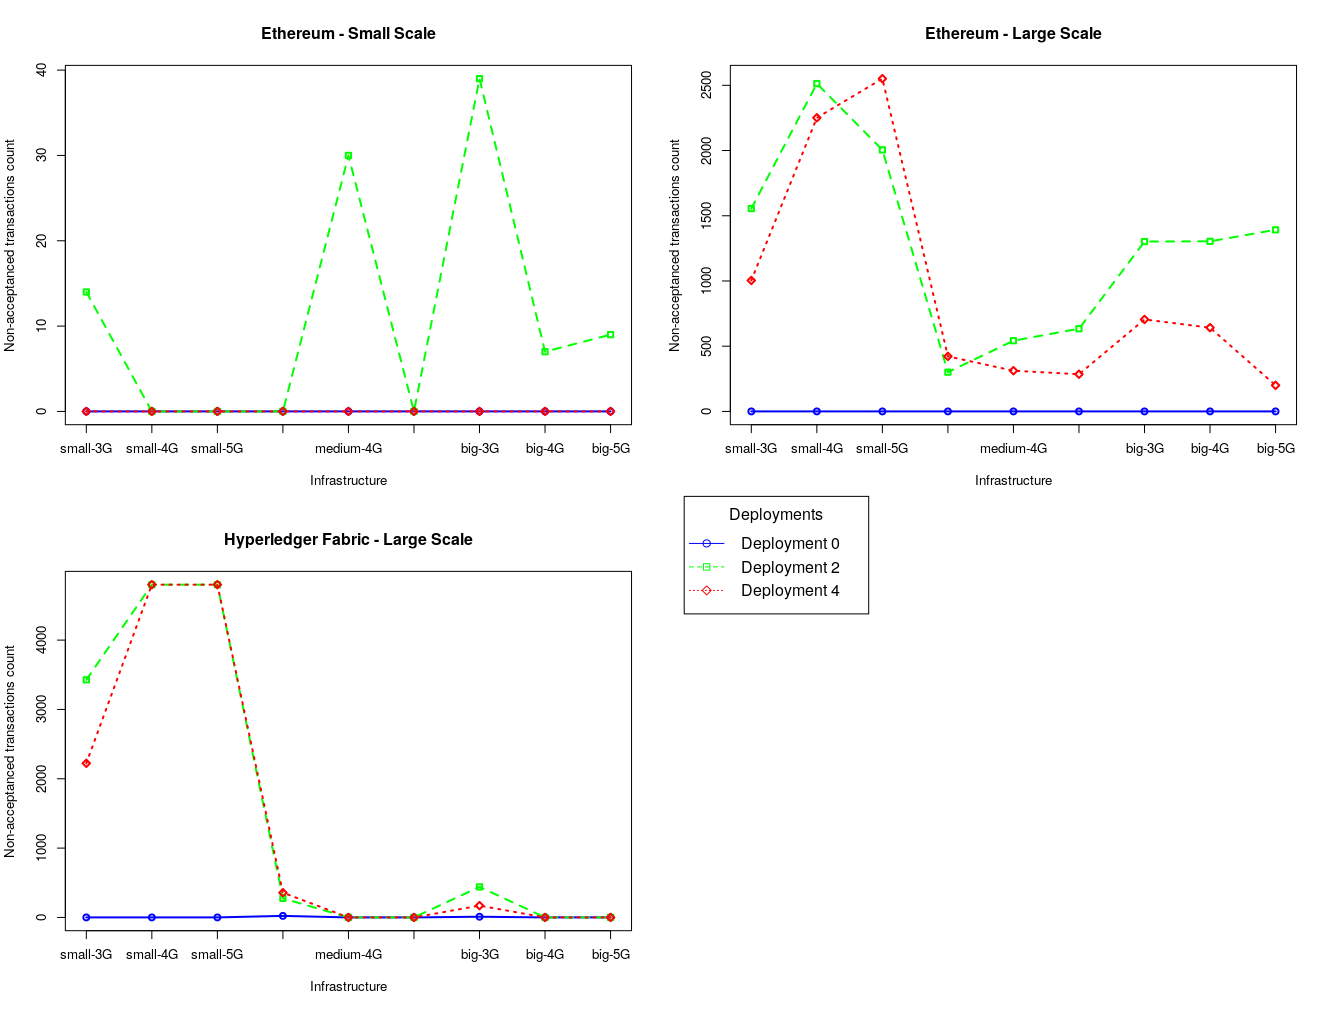
\includegraphics[width=0.8\textwidth]{figures/interaction3_rejected_tx.png}
			\vspace{-0.5cm}
			\caption{Number of rejected transactions in interaction 3 (vehicle-edge node-vehicle)}
			\label{fig:experiments4}
		\end{figure}
	
	\end{frame}

	\begin{frame}
		\frametitle{Experiments}
		
		\begin{figure}
			\centering
			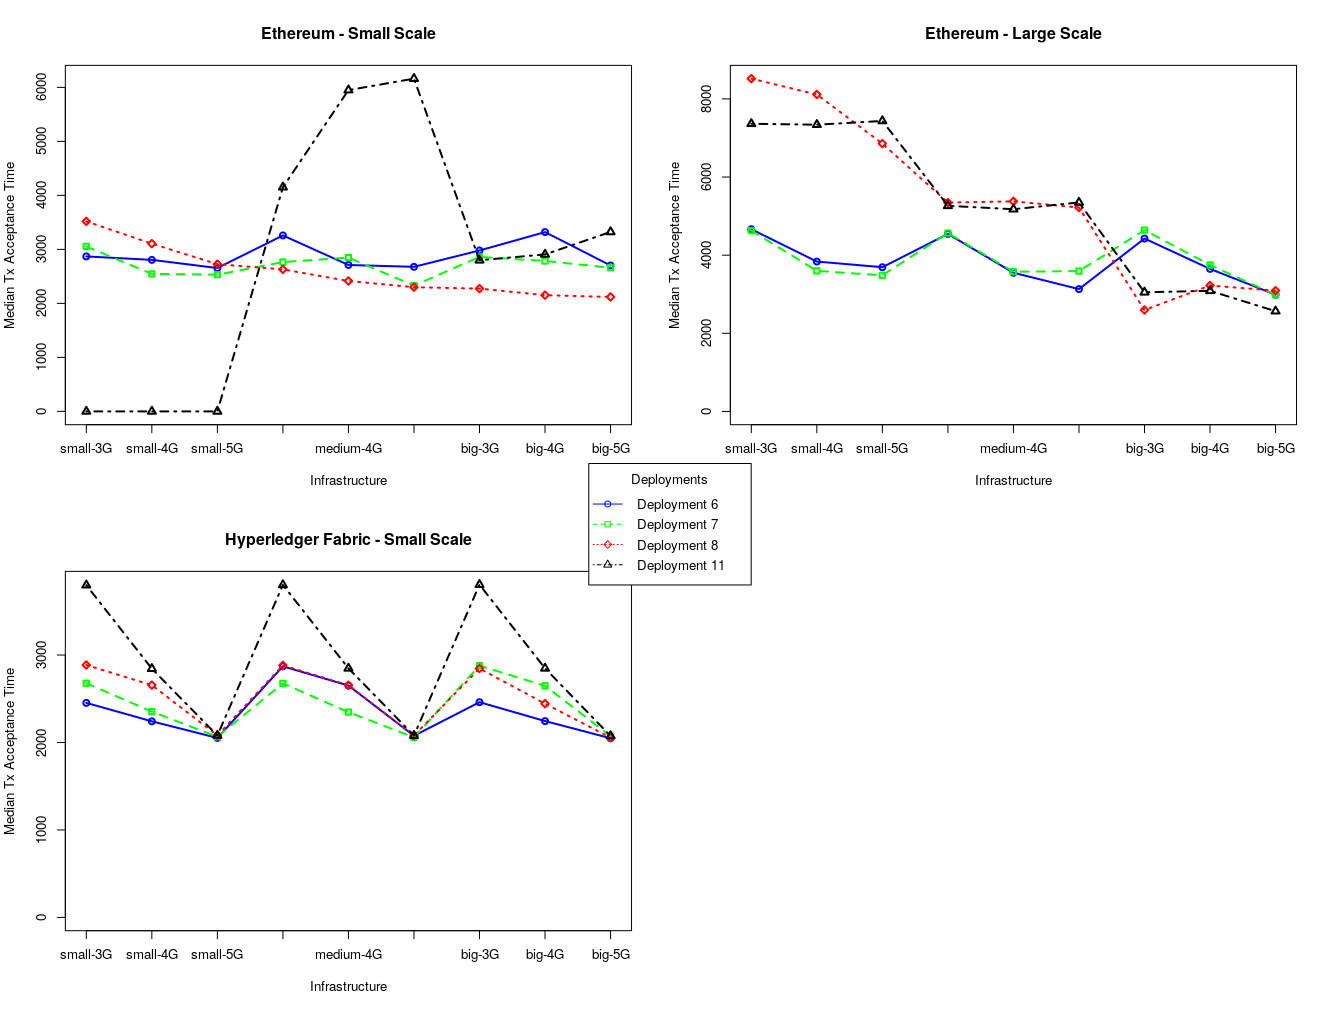
\includegraphics[width=0.8\textwidth]{figures/interaction4_median_accept_time.png}
			\vspace{-0.5cm}
			\caption{Median of transaction acceptance times for interaction 4 (vehicle-\gls{RSU}-edge node-vehicle)}
			\label{fig:experiments5}
		\end{figure}
		
	\end{frame}


	\begin{frame}
		\frametitle{Experiments}
		
		\begin{figure}
			\centering
			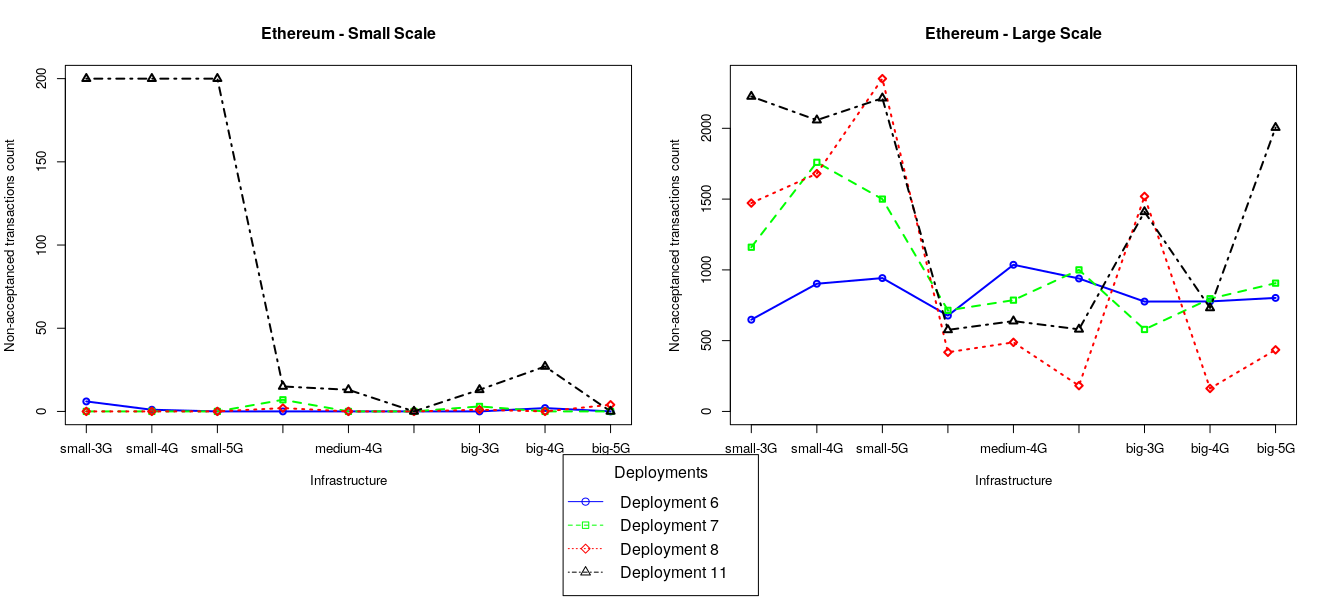
\includegraphics[width=0.8\textwidth]{figures/interaction4_rejected_tx.png}
			\vspace{-0.5cm}
			\caption{Number of rejected transactions in interaction 4 (vehicle-\gls{RSU}-edge node-vehicle)}
			\label{fig:experiments6}
		\end{figure}
	
	\end{frame}

	\begin{frame}
	\frametitle{Features}
	
	
		\begin{itemize}
			\item Sharing benchmarks with the Experiment Knowledge Service.
			\item Search benchmarking interactions, topologies or infrastructures.
			\item Recommend a deployment of blockchain artefacts into a model of application in \gls{MEC}.
			\begin{itemize}
				\item Load application model and preferences on metrics of quality.
				\item Find most similar deployment pattern in the Experiment Knowledge Service.
				\item Find a benchmark of the most similar deployment pattern, for which best results concerning the preferred quality metrics have been measured.
				\item Return a topology of the benchmark.
			\end{itemize}
		\end{itemize}
		
	\end{frame}

	\begin{frame}
		\frametitle{Experiment Knowledge Service - Prototype}
		
		\begin{figure}
			\centering
			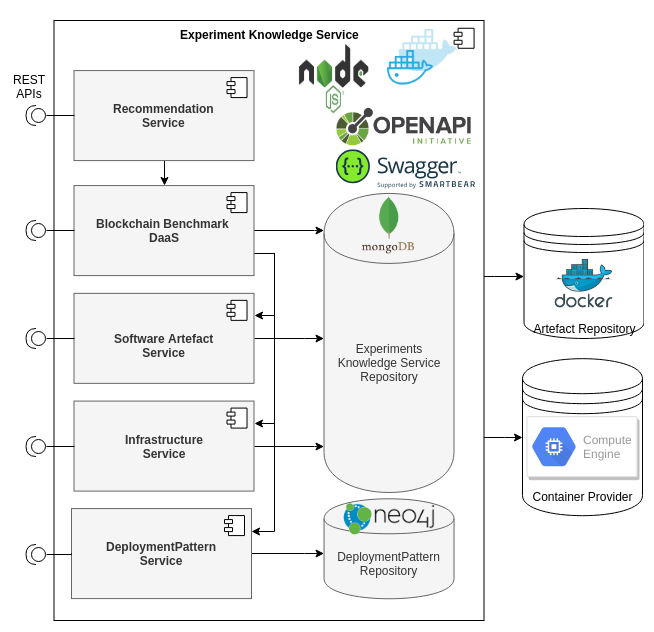
\includegraphics[width=0.6\textwidth]{figures/knowledge_service_architecture_prototype.png}
			\vspace{-0.5cm}
			\caption{Prototype of Experiments Knowledge Service}
			\label{fig:prototype}
		\end{figure}
		
	\end{frame}
	
	
\end{document}